\documentclass[12pt, letterpaper]{article}
\usepackage[utf8]{inputenc}
\usepackage{amsmath, amsfonts, amssymb}
\usepackage{graphicx}
\usepackage[margin=1in]{geometry}
\usepackage{enumitem}
\usepackage{amssymb} 
\usepackage{listings}
\documentclass[12pt, a4paper]{article}
\usepackage[utf8]{inputenc}
\usepackage{geometry}
\usepackage{amsmath}
\usepackage{amssymb}
\usepackage{graphicx}
\usepackage{booktabs}
\usepackage{multirow}
\usepackage{float}
\usepackage{listings}
\usepackage{xcolor}
\usepackage{hyperref}

\geometry{
 a4paper,
 total={170mm,257mm},
 left=20mm,
 top=20mm,
}

\lstset{
    basicstyle=\ttfamily\footnotesize,
    breaklines=true,
    frame=single,
    numbers=left,
    numberstyle=\tiny,
    keywordstyle=\color{blue},
    commentstyle=\color{gray}
}

% Set paragraph indentation and spacing for better readability
\setlength{\parindent}{0pt}
\setlength{\parskip}{1em}

\title{Assignment - 1}
\author{ANANDAN IYER \\ Roll No. : 240117 \\ Department of Mechanical Engineering \\ CGS698C : Bayesian Models and Data Analysis}

\begin{document}

\maketitle

\section*{Part 1 | Sets}

Let $A = \{ x \mid x \in \mathbb{R} \text{ and } -1 \le x \le 2 \}$
\newline
Let $B = \{ x \mid x \in \mathbb{R} \text{ and } 1\le x \le 4 \}$

\begin{enumerate}[label=\alph*)]
    \item $A \cup B = \{ x \mid x \in \mathbb{R} \text{ and } -1 \le x \le 4 \}$
    \item $A \cap B = \{ x \mid x \in \mathbb{R} \text{ and } 1 \le x \le 2 \}$
    \item $A \setminus B = \{ x \mid x \in \mathbb{R} \text{ and } -1 \le x < 1 \}$
    \item $\bar{A} \cap B = \{ x \mid x \in \mathbb{R} \text{ and } 2 < x \le 4 \}$
\end{enumerate}

\section*{Part 2 | Probability}

\textbf{2.1}
Given: $P(H_a) = 0.6$ and $P(H_b) = 0.4$

a) Sample space = $\{ H_aH_b, H_aT_b, T_aH_b, T_aT_b \}$

b) (i) $P(E_1) = P(H_a \cup H_b) = 1 - P(\bar{H_a} \cap \bar{H_b})$
\newline
$P(E_1) = 1 - (0.6 \times 0.4) = 0.76$ 
\newline
\textit{(Note: $1 - P(T_a)P(T_b) = 1 - (0.4)(0.6) = 0.76$)}

(ii) $P(E_2) = P(\bar{H_b} \cap H_a)$
\newline
$= 0.6 \times 0.6 = 0.36$

c) 
$P(H_aH_b) = 0.6 \times 0.4 = 0.24$
\newline
$P(H_aT_b) = 0.6 \times 0.6 = 0.36$
\newline
$P(T_aH_b) = 0.4 \times 0.4 = 0.16$
\newline
$P(T_aT_b) = 0.4 \times 0.6 = 0.24$

The set of probabilities is $\{ 0.24, 0.36, 0.16, 0.24 \}$.

\textbf{2.2}
Sample space $\Omega = \{ (x_1, x_2, \dots, x_5) \mid x_i \ge 0 \text{ for } i=1,2,3,4,5 \}$
\newline
$\Omega_x = \{ 0, 1, 2, 3, 4, 5 \}$

a) Let $w = (x_1, x_2, x_3, x_4, x_5)$ where $x_i$ is the $i^{th}$ margin.
Define an indicator random variable $I$ as:
$I(x_i) = \begin{cases} 1, & x_i \le 5 \\ 0, & x_i > 5 \end{cases}$

Then the random variable is defined as:
$X(w) = \sum_{i=1}^{5} I(x_i)$

b) say $p$ is the probability that the hunter misses by a margin less than or equal to 5 cm.

So, $P(X=k) = \binom{5}{k} p^k (1-p)^{5-k}$ , where k is an integer from 0 to 5 (inclusive)

\section*{Part 3 | Discreet random variables}

\textbf{3.1} Binomial Probability Function: $f(k; n, p) = \frac{n!}{k!(n-k)!} p^k (1-p)^{n-k}$

Given: $p = 0.9$, $k = 45$, $n = 50$

$f(45; 50, 0.9) = \frac{50!}{45! \times 5!} (0.9)^{45} \times (1-0.9)^{5}$

$= 0.18492$

Probability that they will correctly recognize 45 out of 50 words $= 0.18492$

\textbf{3.2} Probability Function: $f(k; \lambda) = \frac{\lambda^k e^{-\lambda}}{k!}$, where $\lambda = 10$.

Probability of 0 accidents in a day ($k=0$):

$f(0; 10) = \frac{10^0 \times e^{-10}}{0!} = e^{-10} = 4.539 \times 10^{-5}$

$f(0; 10) = 4.539 \times 10^{-5}$

\section*{Part 4 | Rate of Covid infections}

\textbf{4.1} Probability of 100 infections in a day $\approx 0$.

\textbf{4.2} $P(5 \text{ to } 15) \sim 0.9220$

\textbf{4.3} $\Omega = \{ x \mid x \in \mathbb{Z}, x \ge 0 \}$ (Set of all positive integers).

\newpage
\textbf{4.4}

\begin{figure}[hbt!]
    \centering
    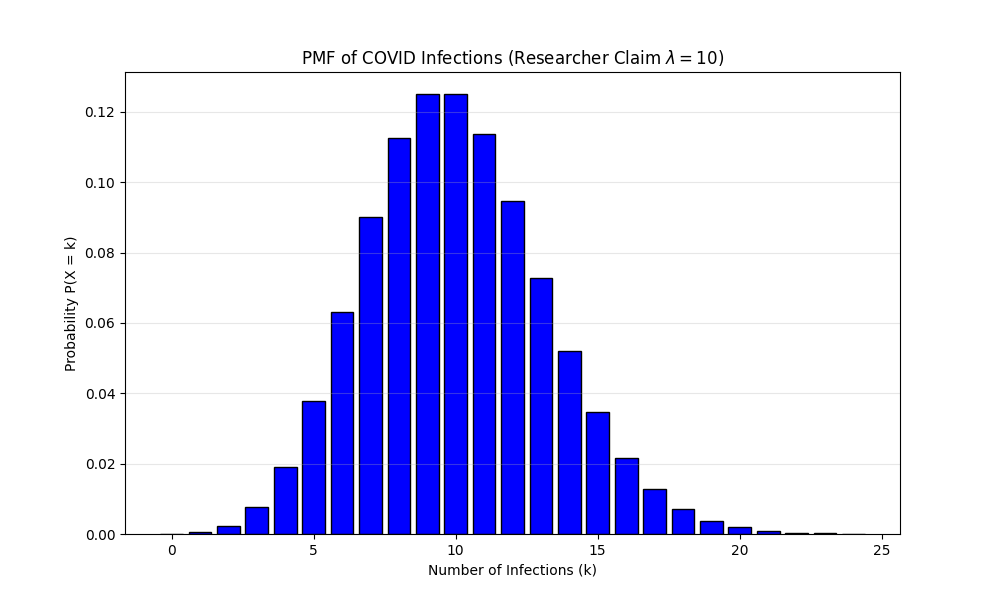
\includegraphics[width=0.8\textwidth]{Figure_1.png} 
    \caption{Graph of the probability mass function}
    \label{fig:section4.4}
\end{figure}
%-------------------------------------------------------------------------


\textbf{4.5} The Researcher is wrong. Actual mean $= 19.4$ while the researcher claimed $\lambda = 10$.
Hence, the generative process claimed does not match reality. \square

\textbf{4.6.1}
First 5 predictions $= [8 \ 12 \ 3 \ 7 \ 14]$
\newline
\textbf{4.6.2}
Next 5 predictions $= [11 \ 15 \ 75 \ 12 \ 10]$

Hence, the 2 sets of predictions are not the same. \square

\newpage
\section*{References}

\begin{lstlisting}[language=Python]
import numpy as np
import matplotlib.pyplot as plt
from scipy.stats import poisson

lambda_ = 10 

prob2 = poisson.pmf(100, lambda_)
prob1 = sum(poisson.pmf(k, lambda_) for k in range(5, 16))

k_values = np.arange(0, 25)

pmf_values = poisson.pmf(k_values, lambda_)

plt.figure(figsize=(10, 6))
plt.bar(k_values, pmf_values, color='blue', edgecolor='black')
plt.title(f'PMF of COVID Infections (Researcher Claim $\lambda={lambda_}$)')
plt.xlabel('Number of Infections (k)')
plt.ylabel('Probability P(X = k)')
plt.grid(axis='y', alpha=0.3)

actual_data = [18, 20, 23, 25, 22, 30, 11, 10, 23, 12]
actual_mean = np.mean(actual_data)

predictions_1 = poisson.rvs(lambda_, size=5)
predictions_2 = poisson.rvs(lambda_, size=5)

print(f"Part 4")
print(f"4.1: Probability of 100 infections: {prob2:.50f}")
print(f"4.2: Probability between 5 and 15: {prob1:.4f}")
print(f"4.5: Calculated Mean: {actual_mean} vs Researcher's Mean: {lambda_}")
print(f"4.6.1: First 5 predictions: {predictions_1}")
print(f"4.6.2: Next 5 predictions:  {predictions_2}")
print(f"Are they the same? {'Yes' if np.array_equal(predictions_1, predictions_2) else 'No'}")
plt.show()
\end{lstlisting}

\end{document}